

\documentclass[10pt, conference, compsocconf]{IEEEtran}

\usepackage[utf8]{inputenc}
\usepackage[american]{babel} 

\usepackage{graphicx}
\usepackage{float}

\graphicspath{{figures/}}
\DeclareGraphicsExtensions{.pdf,.PDF,.png,.PNG}  

\let\labelindent\relax
\usepackage{enumitem}

\usepackage{csquotes}
\usepackage{xcolor} 
\usepackage{csquotes}

\usepackage[draft]{hyperref}

\ifCLASSINFOpdf
\else
\fi

\renewcommand{\sectionautorefname}{Section}
\renewcommand{\figureautorefname}{Fig.}

\definecolor{cardinal}{rgb}{0.77, 0.12, 0.23}
\newcommand{\redify}[1]{\textcolor{cardinal}{#1}}
\definecolor{cobalt}{rgb}{0.0, 0.28, 0.67}
\newcommand{\blueify}[1]{\textcolor{cobalt}{#1}}

\renewcommand{\descriptionlabel}[1]{\hspace{\labelsep}\textbf{#1} |}


\usepackage{listings} 
\usepackage{accsupp}

% This ensures numbers are not copied, but leading spaces are copied, as taken from
% http://tex.stackexchange.com/a/30310

\newcommand{\noncopynumber}[1]{%
    \BeginAccSupp{method=escape,ActualText={}}%
    #1%
    \EndAccSupp{}%
}

\makeatletter
\def\lst@outputspace{{\ifx\lst@bkgcolor\empty\color{white}\else\lst@bkgcolor\fi\lst@visiblespace}}
\makeatother

\definecolor{msvc_keyword}   {HTML}{0000FF} 
\definecolor{msvc_comment}   {HTML}{008000} 
\definecolor{msvc_background}{HTML}{eff0f1} 
\definecolor{msvc_frame}     {HTML}{EAEAEA}
\definecolor{msvc_linenumber}{HTML}{2B91AF}
\definecolor{msvc_string}    {HTML}{A31515}

\definecolor{msvc_directives}{HTML}{808080}
\definecolor{msvc_operators} {HTML}{2B91AF}
\definecolor{msvc_stl}       {HTML}{2B91AF}

\lstdefinelanguage{TypeScript}
{
    keywords        = {break, case, catch, continue, debugger, default, delete, do, else, finally, for, function, if, in, instanceof, new, return, switch, throw, try, typeof, var, void, while, with, super, class, constructor},
    morecomment     = [l]{//},
    morecomment     = [s]{/*}{*/},
    morestring      = [b]',
    morestring      = [b]", 
    keywordstyle    = \color{blue}\bfseries,
    identifierstyle = \color{black},
    commentstyle    = \color{teal}\ttfamily,
    stringstyle     = \color{red}\ttfamily,
    sensitive       = true,
    style           = TypeScript
}

\lstdefinestyle{TypeScript}
{
    basicstyle       = 
\ttfamily
\lst@ifdisplaystyle\footnotesize\fi %
,   backgroundcolor  = \color{msvc_background}
,   rulecolor        = \color{msvc_background}
,   keywordstyle     = \lst@ifdisplaystyle\color{msvc_keyword}\fi
,   commentstyle     = \lst@ifdisplaystyle\color{msvc_comment}\fi
,   stringstyle      = \lst@ifdisplaystyle\color{msvc_string}\fi
,   showstringspaces = false
,   numberbychapter  = true
,   numbersep        =  8pt
,   showlines        = true
,   tabsize          =  4          
,   numbers          = left
,   numberstyle      = \tiny\color{msvc_linenumber}\noncopynumber
,   framesep         =  4pt
,   xleftmargin      = \parindent
,   xleftmargin      = 16pt
,   framexleftmargin = 16pt
,   abovecaptionskip = \medskipamount
,   stepnumber       = 1
,   columns          = flexible
,   keepspaces       = true
,	keywords         = [2]{ prototype, this }
,	keywordstyle     = [2]\lst@ifdisplaystyle\color{msvc_stl}\fi
,   morekeywords     = [1]{ noexcept }
,	literate         = *
{[}{{\lst@ifdisplaystyle\color{msvc_operators}\fi{[}}}{1}
{]}{{\lst@ifdisplaystyle\color{msvc_operators}\fi{]}}}{1}
}


\hyphenation{op-tical net-works semi-conduc-tor}

\makeatletter
\g@addto@macro\@maketitle{
    \vspace{-1\baselineskip}
    \vspace{1.6\baselineskip}
    \begin{figure}[H]
        \setlength{\linewidth}{\textwidth}
        \setlength{\hsize}{\textwidth}
        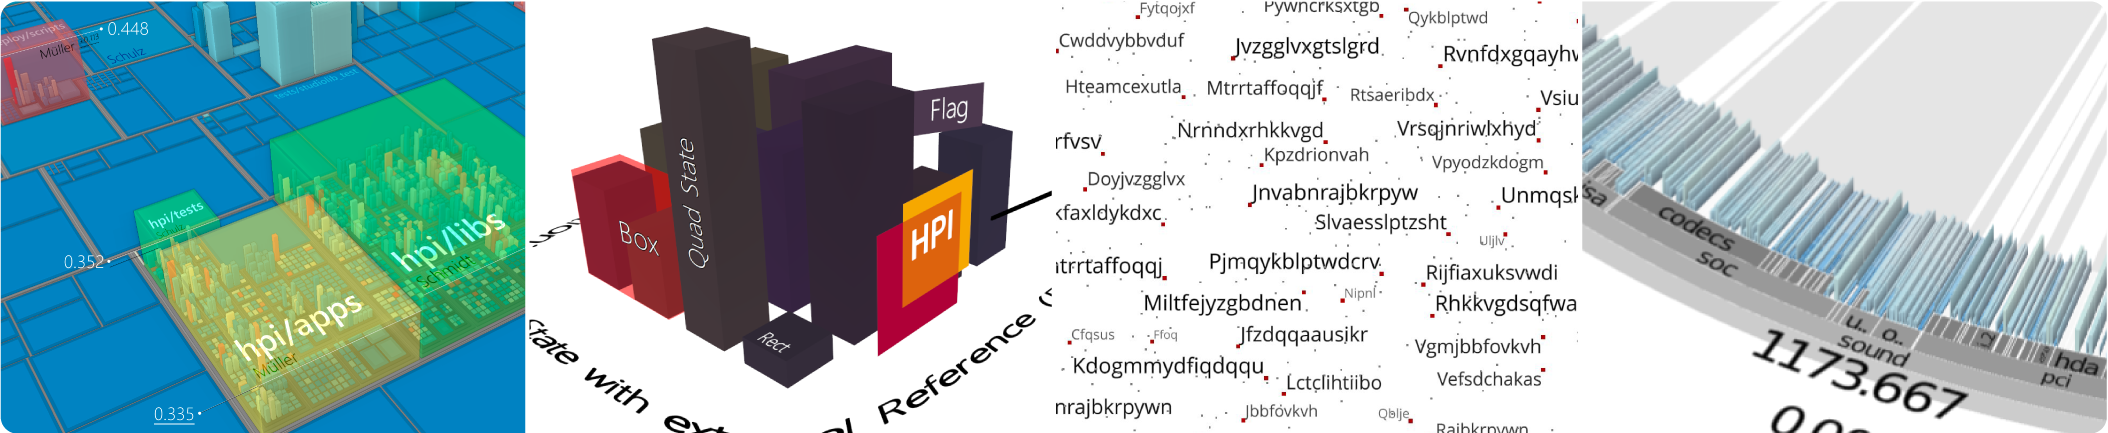
\includegraphics[width=\textwidth]{teaser2}
        \caption{fltr, a data visualization using interactive annotation, a synthetic scene showcasing automatic label placement, a benchmark for point-feature label placement, and a circular bundle view using labeling with adaptive level-of-detail, automated label orientation as well as text-alignment along B-splines.}
        \label{fig:teaser}
    \end{figure}
}
\makeatother

\usepackage{eso-pic}
\AddToShipoutPictureFG{\AtPageLowerLeft{\put(\LenToUnit{0.5\paperwidth},\LenToUnit{6mm}){\makebox[0pt][c]{\fontsize{6.5}{8}\selectfont\color{gray}Author's revised version (2026-11-12). Version of record: \url{https://doi.org/10.1109/iV.2018.00039}}}}}
\begin{document}
\title{OpenLL: an API for Dynamic 2D and 3D Labeling}

\author{\IEEEauthorblockN{Daniel Limberger\IEEEauthorrefmark{1}, Anne Gropler, Stefan Buschmann, and J{\"u}rgen D{\"o}llner\IEEEauthorrefmark{2}}
\IEEEauthorblockA{Hasso Plattner Institute, University of Potsdam\\
Potsdam, Germany\\
Email: \{daniel.limberger\IEEEauthorrefmark{1}, juergen.doellner\IEEEauthorrefmark{2}\}@hpi.de}
\and
\IEEEauthorblockN{Benjamin Wasty\IEEEauthorrefmark{3}}
\IEEEauthorblockA{Seerene\\
Potsdam, Germany\\
Email: benjamin.wasty@seerene.com\IEEEauthorrefmark{3}}
}

\maketitle

\begin{abstract}
  Today's rendering APIs lack robust functionality and capabilities for dynamic, real-time text rendering and labeling, which represent key requirements for 3D application design in many fields.
  As a consequence, most rendering systems are barely or not at all equipped with respective capabilities.
  This paper drafts the unified text rendering and labeling API OpenLL intended to complement common rendering APIs, frameworks, and transmission formats.
  For it, various uses of static and dynamic placement of labels are showcased and a text interaction technique is presented.
  Furthermore, API design constraints with respect to state-of-the-art text rendering techniques are discussed.
  This contribution is intended to initiate a community-driven specification of a free and \emph{open label library}.
\end{abstract}

\begin{IEEEkeywords}
visualization, labeling, real-time rendering
\end{IEEEkeywords}

\IEEEpeerreviewmaketitle


\section{Introduction}
\label{sec:introduction}
\noindent
\enquote{A major limiting factor to the widespread use of information visualization is the difficulty of labeling information abundant displays}~\cite{Fekete1999}.
This assessment of Fekete and Plaisant is as tenable today as it was in 1999.
Most of today's visualizations are still troubled by missing labels, leading to one-by-one assessment of graphical elements, overlapping labels obscuring depicted data, and ambiguous association of labels to graphical elements.
Even recent advances in big-data visualization have not managed to resolve these well-known labeling issues, despite their tremendous potential for increasing the visualization quality. 

We suppose there are at least two reasons for labeling to remain mostly unattended in real-time computer graphics.
First, high-quality text rendering and placement is an intricate task, especially in 3D. 
It starts with text rendering itself requiring lots of implementation and use-case specific tweaking and probably ends with having no text rendering support in any of the latest rendering APIs, be it OpenGL~\cite{opengl}, WebGL~\cite{webgl}, or Vulkan~\cite{vulkan}.
In research, this means lots of available resources ought to be allocated for prototype development rather than novelty and evaluation.
Second, other industries, like the gaming industry usually get along with basic (bitmap based) text rendering.
With a few exceptions (e.g., \emph{Tom Clancy's The Division}, developed by Massive Entertainment and published by Ubisoft in 2016, shows impressive dynamic labeling in its UI and world map), high-end labeling is attributed to artistic rather than programming efforts and is the result of tweaking and pre-computing assets in compliance with a title's art direction.
Furthermore, the number of labels is typically much smaller and sophisticated placement requirements are not present. 
Accordingly no industry seems to drive the progression or standardization of labeling technology in general.

In order to initiate a research driven specification of an open label library, we (1) put our idea of a unified labeling API forward for discussion, and (2) propose subsequent steps required for a widespread use in information visualization.
To this extent, the following contributions are made: %
\begin{itemize}
	\item a brief introduction to and overview of existing text rendering approaches and systems is provided,
	\item snippets of the labeling API \emph{OpenLL}, derived from use cases of our research group, are presented, and
	\item our ongoing open-source implementation efforts for mobile and desktop applications are described.
\end{itemize}

\smallskip
\noindent
OpenLL is designed to complement existing rendering APIs, systems, and transmission formats (such as glTF~\cite{gltf}).
It facilitates a descriptive labeling approach using label and proxy objects that are processed by means of renderers that are aligned to implementation specifics of hardware-accelerated text rendering techniques.
Thus, this paper provides the general concepts of OpenLL instead of drafting an extension to any rendering API or transmission format.


\section{Related Work}
\label{sec:related}
\noindent
This section covers related work in the fields of text rendering techniques and systems, and labeling in information visualization in general. 

\subsection{Text Rendering Techniques}
\noindent
With OpenLL we are targeting real-time rendering scenarios in which any additional processing might impact the overall rendering performance or interaction experience.
This means that rendering hundreds of labels within a virtual reality application at 90\,Hz or higher, for example, constrains the available processing time for labeling within each frame to at the very most a millisecond. 
Accordingly, the best practice for increasing real-time rendering performance is often to \enquote{avoid text rendering whenever possible}\footnote{Performance tips for using the canvas: \url{https://developer.mozilla.org/en-US/docs/Web/API/Canvas_API/Tutorial/Optimizing_canvas}}.
To counter this practice, OpenLL is specifically aligned to text rendering techniques that take advantage of texture-mapping graphics hardware by using bitmaps, signed distance fields, and vector maps.

Bitmap font
    rendering is the basis for rendering dynamic text, i.e., text that can change at run-time and cannot be prerendered into a texture. 
    The text is divided into its elemental symbols (\emph{glyphs}), each represented by a quad and typeset (using additional kerning data or monospace) on the CPU.
    Each glyph's coverage values are prerendered into a bitmap using, e.g., FreeType~\cite{freetype1996} or quadratic curve evaluation~\cite{Wallace2016}, and packed into a texture map.
    The GPU is then used to texture every glyph using its respective subregion within the texture map.
    This approach is feasible as long as the text is displayed at a fixed size in pixels.

Signed distance fields (\emph{SDF})
    representing the glyphs' shapes can be used to better account for varying display resolution as well as text size and orientation~\cite{Frisken2000}.
    Each distance function is sampled and encoded as a bitmap within the texture map.
    The GPU can then reconstruct a glyph's shape at any orientation by interpolating bilinearly and thresholding the distances.
    Furthermore, per-pixel screen-space derivatives can be used to properly anti-alias the glyph edges~\cite{Qin2006} and multiple texture channels, representing different edges intersecting within a texel, can be used in order to preserve sharp corners~\cite{Green2007}.

Spline fragment-based sampling approaches were recently considered to fully overcome all limitations of the bitmap and SDF based approaches.
    Quadratic B\'ezier curve segments for every glyph are efficiently encoded in a texture.
    This data is then decoded and locally supersampled per fragment on the fly \cite{Dobbie2016}.
    \enquote{It should be clear that [this approach] requires considerably more computation}~\cite{Lengyel2017} (and dependent texture lookups) in comparison to SDF.
    However, this approach is still fast enough to enable rendering of many labels in real-time while providing the most flexibility and best quality.

\subsection{Text Rendering Systems}
\noindent
The presented API requires text to be placed and transformed in virtual two- and three-dimensional scenes. 
Text rendering facilities exposed via native GUI APIs such as \emph{Core Text}, \emph{Direct Write}, Windows \emph{GDI}, \emph{Qt}, \emph{X11}, or \emph{Xft} are usually tightly integrated into a framework or operating system. 
For the most part, though supporting hardware acceleration, they cannot be used from within custom hardware-accelerated contexts nor be non-trivially transformed.
 
Font rendering libraries such as FreeType~\cite{freetype1996} are focusing on handling font faces, typesetting, and text rendering in 2D and can be used, e.g., to prerender glyphs to textures for hardware-accelerated use.
One promising library for fast text rendering using OpenGL is \emph{freetype-gl}~\cite{freetypegl2011}; however, there are no means for advanced placement and arbitrary transformations yet.

For web applications targeting browsers there is a similar lack of support. 
Even though browsers have advanced text rendering capabilities, they are not fully exposed to developers.
The rendering library \emph{three.js}~\cite{cabello2010} creates vertex-based geometry for text rendering (there are community examples showing SDF rendering that use three.js's text capabilities though) and suggests HTML or canvas rendering for the visual display of large amounts of text.
With CSS 3 and HTML one could achieve adequate 2D and 3D transformed labeling by creating a pool of HTML text elements and changing their position and content dynamically~\cite{limberger2013}.
This, however, does not allow for occlusion by the 3D scene (e.g., shared depth buffer) and yields inefficient rendering performance.

\subsection{Labeling in Information Visualization} 
\noindent
OpenLL is intended as an extensible API covering various labeling approaches.
Kakoulis and Tollis provide a good introduction to and overview of labeling problems that were identified within the context of cartography and rendering maps~\cite{Kakoulis2013}.
Labeling techniques can be categorized as internal or embedded~\cite{Maass2007}, external, boundary, and excentric labels~\cite{Oeltze-Jafra2014}.
For their placement, various quality measures and requirements are commonly applied:
(1) readability w.r.t. overlap, orientation, and occlusion with other graphical elements, 
(2) unambiguity w.r.t. the referenced/associated graphical element(s), 
(3) minimization of visual clutter, 
(4) eligibility for dynamic placement in real-time,
(5) temporal coherence by means of reducing visual discontinuities, and, finally, their
(6) compaction, i.e., the minimization of each individual layout area itself~\cite{Ali05}.
In addition, problem- and computation-specific measures and constraints, e.g., attractive and repulsive forces~\cite{Balata2014} might be introduced.

A vast number of labeling placement techniques such as positioning names on maps~\cite{Imhof1975}, point feature label placement~\cite{Christensen1995}, external label management in 3D object space~\cite{Tatzgern2014}, or force-based labeling~\cite{Vaaraniemi2012} have been introduced.
Furthermore, the labels themselves can be used as proxies for interaction as shown by, e.g., Balata et al.~\cite{Balata2014}.
For the design of OpenLL this necessitates extension points that account for and embrace the diversity of application domains and labeling approaches.


\section{Labeling Model}
\label{sec:model}
\noindent
The core of our labeling API is about management and automated placement of a large number of labels in 2D and 3D in real-time.
It does not provide implementation specifics, e.g., for computational math, parallelization, or hardware accelerated rendering, nor does it impose a certain implementation design.
However, for deriving font handling interfaces and general rendering features it is relevant to account for common limitations of today's rendering approaches.
Similar to rendering APIs we expose objects and operate on the object relations and states.
For it, we introduce the following API objects:\medskip

\begin{description}\setlength{\itemsep}{8pt}

	\item [Font Face]
	The font face describes the resources required for rendering text. This includes, e.g., a list of available glyphs and ligatures, their orientation, advance, weight, and kerning data, their location within a texture map as well as the texture map's encoding, e.g., 16-bit floating-point SDF samples or 8-bit RGBA coverage.
	We assume all assets to be generated beforehand, but a font family reference could also be used if the OpenLL driver is capable of generating the required assets on the fly. 
	
	\item [Text]
	This object stores the actual text by means of a dynamic sequence of characters or code points.
	
	\item [Label]
	A label combines all data required for typesetting, positioning, orienting, and rendering text.
	It references a text or an excerpt of a text, a font face and style definition, and describes its specific placement via positions, margins, anchors, proxies, constraints, or auxiliary shapes such as lines, points, etc.
	It also represents the main extension point for domain-specific labeling techniques.
	
	\item [Label Cloud]
	This object can be used for data-driven labeling, e.g., when a large number of points or objects are selectively labeled based on weights or other label-specific data.
	For that, the text references, placement and weight data must be provided. 
	The font face and style definitions are referenced only once, and depending on the cloud's specialization, additional data such as a label selection description, maximum number of labels to be displayed, or no-label regions can be added.

	\item [Proxy]
	Similar to real-time collision physics, implicit shapes like spheres, cubes, quads, points, lines, or splines can be used to partially approximate detailed 2D and 3D scenes or describe dynamic anchors such as a virtual camera or an area of interest.
	With this, the computational complexity of label placement and anchoring, especially for more advanced, e.g., constraint-based, adaptive label placement techniques can be reduced.
	Any label can then reference a proxy's vertices, edges, or areas as an anchor. 
	For example, a cuboid proxy could expose each of its corners, edges, center points, or even its lateral surfaces for anchoring. 
	Proxies also provide the basis for detecting overlapping labels, adapting to proxies occluding labels, or using their extent for level-of-detail control.

	\item [Renderer]
	The renderer is tasked with configuration, preparation and real-time rendering of a given set of labels or label clouds.
	There might be various rendering implementations favoring specific text rendering approaches or font assets.
	OpenLL does not assume any rendering implementation details, and instead provides, if any, generic quality and performance hints, e.g., flags for favoring quality over memory.
	It is the renderer's responsibility to internally gather data such as device pixel ratios for correct font size scaling and display sub-pixel layout for sub-pixel anti-aliasing.
	Finally, the renderer must allow label retrieval via screen space coordinates for user interaction purposes.

\end{description}

\smallskip
\noindent
Using these objects, the general approach for rendering labels is as follows: (1) prepare font faces and proxies, (2) instantiate labels or label clouds, (3) configure one or multiple renderers and callbacks, and, finally, (4) update texts and proxies and trigger the rendering on every frame.
The actual placement of the labels should be triggered by the renderer internally in the following manner:
all labels and clouds that are about to be rendered are triggered for a lazy update. If any of their properties or referenced objects (font face, proxies, etc.) has changed, all required transformations for placement and rendering are (re)computed and associated geometry (re)submitted for rendering.

Overall, this design facilitates a community-driven standardization of 2D and 3D labeling by means of extensions, facades, or new libraries, and thus promotes the use of existing text rendering engines, e.g., \emph{glyphy}~\cite{Esfahbod2011}, \emph{freetype-gl}~\cite{freetypegl2011}, \emph{FreeType}~\cite{freetype1996}, or even native frameworks.  


\section{Labeling API}
\label{sec:api}
\noindent
This section discusses the labeling API by examples derived from use cases in the fields of Geovisualization and Software visualization. The examples are in pseudocode, but the syntax is inspired by TypeScript for readability.

\subsection{Basic Label Placement in 2D}
\noindent
The first listing shows how to create and render a single 2D label, specifying basic font and placement options:

\lstinputlisting[language = TypeScript, label = lst:basic2d]{listings/basic2d.js}

\noindent
The options can be specified declaratively by passing a JSON object to the label constructor, but also changed procedurally later (line 12). 
They are loosely based on CSS rules where possible.
For example, the font face can be specified as a relative path to a file. %
There are also options for the renderer that can be set dynamically, such as supersampling using RGSS (\textit{rotated grid supersampling}).  

\subsection{Multi-line Labels in 2D}

\noindent
This example shows a multi-line label that is rendered into a given rectangle, specifying word wrap, overflow behavior, and padding in a similar manner to CSS.
This allows, e.g., for labeling proxy objects such as faces of a bounding box:

\lstinputlisting[language = TypeScript, label = lst:block2d]{listings/block2d.js} 

\subsection{Label at 3D Position}
\begin{figure}[h]
	\vspace*{-0.75\baselineskip}
	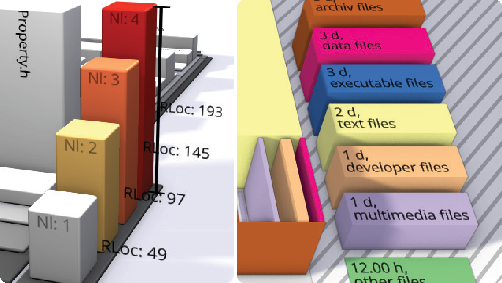
\includegraphics[width=\linewidth]{labeling-in-3d-legends}
	\vspace*{-1.0\baselineskip}
	\label{fig:legends}
\end{figure}
\noindent
This is a basic example of static label placement in 3D space. Contrary to 2D space, we cannot use pixel or point as a unit for font size and positioning, since the actual size of a label depends on its position and the position of the camera. Thus there is no purpose in using any unit other that world space coordinates for font size and positioning:

\lstinputlisting[language = TypeScript, label = lst:position3d]{listings/position3d.js}

\subsection{2D Projected Label at 3D Position}
\begin{figure}[h]
	\vspace*{-0.75\baselineskip}
	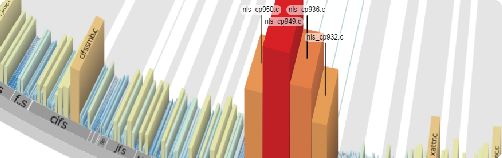
\includegraphics[width=\linewidth]{labeling-poles-adaptive}
	\vspace*{-1.0\baselineskip}
	\label{fig:lineLabel}
\end{figure}
\noindent
Projected 3D labels are positioned in 3D space, but projected onto a 2D plane. The model view projection is used to position the label based on its anchor point that is specified in world coordinates, while the label itself is treated as 2D:

\lstinputlisting[language = TypeScript, label = lst:projected3d]{listings/projected3d.js}

\subsection{Labeling along 3D Splines}
\begin{figure}[h] 
	\vspace*{-0.75\baselineskip}
	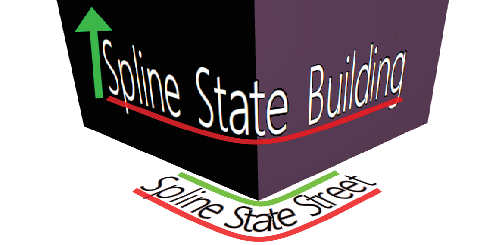
\includegraphics[width=\linewidth]{labeling-spline}
	\vspace*{-1.0\baselineskip}
	\label{fig:building3dspline}
\end{figure}
\noindent
Splines can be useful, e.g., for annotating a 3D-building by wrapping a label around the walls or for labeling a river.
A spline has several properties: control points, knot values and degree. Two of them must be given for defining the spline, the third can be calculated.
For every glyph on a spline, the same up vector can be used. However in 3D space, the up vector can also be different for every glyph. In addition to the base spline (that is the baseline in typesetting), a top spline is defined, which is used to calculate an up vector for every glyph. That up vector is defined by the position of the glyph on the base spline and the corresponding position on the top spline:

\lstinputlisting[language = TypeScript, label = lst:spline3d]{listings/spline3d.js}

\subsection{Adaptive Label Placement}
\noindent
To maintain readability for rendered glyphs, their placement should adapt to changes of view or occluding geometry. When annotating a point, the label can be placed at different angles; when annotating a line, the label can be written over any part of the line -- to mention a few scenarios. We address those issues with two examples, based on uses cases in Treemap-based software visualizations:\medskip

\subsubsection{Adaptive Label Placement in Screen Space}
\noindent
The first example shows an external label in screen space. It uses a line in world space to connect the label to the corresponding object. Changing the view might later result in changing the line origin and thus changing the label position.
\begin{figure}[h]
	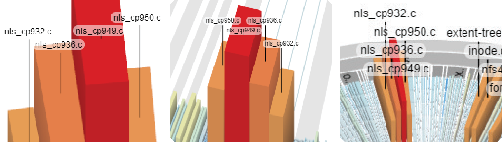
\includegraphics[width=\linewidth]{labeling-adaptive}
	\vspace*{-1.0\baselineskip}
	\label{fig:adaptiveLabelPlacement}
\end{figure}

\subsubsection{Adaptive Label Placement using a Box Proxy}
\begin{figure}[h]
	\vspace*{-0.75\baselineskip}	
	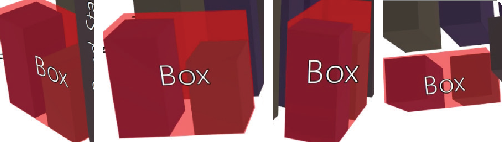
\includegraphics[width=\linewidth]{labeling-box-proxy}
	\vspace*{-1.0\baselineskip}
	\label{fig:boxRef}
\end{figure}
\noindent
The second example uses a proxy in form of a box. Different surfaces of the box are usable for the label's position. It also possible to change the direction and up vector of the label accordingly. At this point, a smart placement algorithm can be interposed to calculate the label's placement taking into account the proxy geometry, the current view, or occluding geometry:

\lstinputlisting[language = TypeScript, label = lst:proxygeom3d]{listings/proxygeom3d.js}

\subsection{Labeling with Level Of Detail} 
\begin{figure}[h]
	\vspace*{-0.75\baselineskip}
	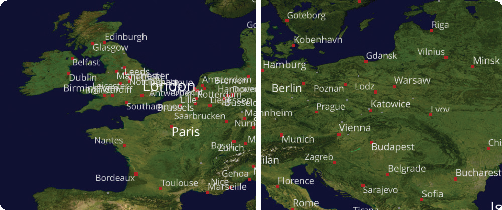
\includegraphics[width=\linewidth]{labeling-cloud-lod}
	\vspace*{-1.5\baselineskip}
	\label{fig:cloud}
\end{figure}
\noindent
When rendering a large amount of labels, the view is easily cluttered and labels overlap or occlude other objects. To prevent that, it is possible to choose a subset of all labels based on certain constraints, e.g., only the 20 most important labels (criterion: label priority or weight), a minimum font size (view-based in 3D), or only certain semantic groups that can have precedence for visual display over other groups.

The following example shows how to define such a label cloud, where multiple labels with the same positioning and stylization properties are gathered. Constraints of different types are added that are evaluated before the labels are rendered:

\lstinputlisting[language = TypeScript, label = lst:projected3d.multiple]{listings/projected3d.multiple.js}



\section{Towards an Open Labeling Library}
\label{sec:openll}
\noindent
The fast and widespread adoption of Vulkan~\cite{vulkan} and glTF~\cite{gltf} are two recent examples of successful introductions of free and open standards.
To address industry and community needs, it is crucial not only to provide plain specifications, but to set up infrastructural means that facilitate adoption by enabling developer feedback, and providing comprehensive documentation, design guidelines and lots of examples.
Most importantly though, we consider the availability of free and open-source reference implementations as well as tools for font-asset generation and API validation to be crucial for a successful adoption of an open label library.

Though not directly intended as an extension to a specific transmission format or rendering API, the presented labeling library is designed to fit today's ecosystem of graphics rendering APIs and real-time rendering techniques.
It should provide reference implementations targeting various rendering APIs from the start.
We are currently focusing on a TypeScript-based WebGL as well as a C++-based OpenGL implementation, but are committed to subsequent ports targeting OpenGL ES and Vulkan in the future.
Both renderers are capable of laying out and rendering thousands of glyphs within a fraction of a millisecond using one of multiple rendering backends (bitmap, SDF, and spline fragments).

As of writing this paper, there is a limited number of robust font asset formats and generators available.
Our reference implementation relies on the quasi-standard bitmap font format\footnote{\url{http://www.angelcode.com/products/bmfont/}} which can be easily extended.
In order to generate font assets we used well-known font generators such as \emph{Hiero} or \emph{Littera} (deprecated due to Adobe Flash).
Due to several shortcomings, we started development of an extensible, free and open-source font-asset generator that features
\begin{itemize}
	\item interactive text rendering preview in 2D and 3D for efficient iterative font asset refinement,
	\item C++ implementation for fast texture packing, signed distance field computation and glyph rasterization~(\autoref{fig:openfag}),
	\item use via command line interface, via integration as library, or via its graphical user interface on all major platforms.
\end{itemize}

\begin{figure}[ht]
	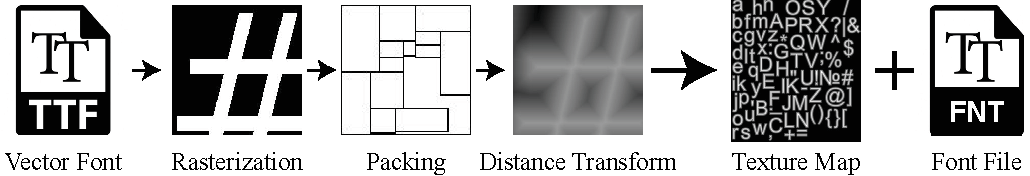
\includegraphics[width=\linewidth]{openfag}
	\vspace*{-1.5\baselineskip}
	\caption{Processing pipeline of our font asset generation library.}
	\label{fig:openfag}	
\end{figure}
 
\section{Conclusion and Future Work}
\label{sec:conclusion}
\noindent
In this paper we presented a draft for an open label library, \emph{OpenLL}, an API that is designed to complement existing rendering APIs, frameworks, and transmission formats.
To this end the API provides key objects, i.e., proxies and labels, for configuration and management of labels in 2D and 3D in real-time.
Proxies can be used to approximate a virtual scene and provide various anchors that are then referenced by labels for placement.
The label itself provides (1) a detailed description of the font face and the actual text for rendering, and (2) the API's main extension point for various types of label placement techniques.
In order to facilitate adoption and community feedback, the API design does not limit the text rendering driver to a specific set of techniques, even though the OpenLL is intended to be used in interactive rendering applications.
Our free and open-source resources~\cite{openll2018}, as partially presented, comprises (1) two reference implementations of the depicted API examples using WebGL and OpenGL and (2) a cross-platform font asset generator.

Both our implementations currently do not support ligatures, composite code points, or more sophisticated typesetting. 
Furthermore, we would like OpenLL to support extruded 3D text (as in \emph{three.js}) and CSS-like stylization options (gradient, outlines, glow, drop shadows, and more).
Finally, we hope this work inspires a community effort, especially in the field of information visualization, towards creating more accessible and unified labeling systems.


\section*{Acknowledgment}
\noindent
The authors would like to thank Daniel Gimbatschki and Simon Krogmann for their valuable API design and implementation contributions.
This work was funded by the German Federal Ministry of Education and Research (BMBF) within the BIMAP project (\url{https://www.bimap-project.de}).

\bibliographystyle{IEEEtran}
\bibliography{references}  

\end{document}

